\documentclass[a4paper,12pt]{article}
\usepackage{indentfirst}
\usepackage[latin1,utf8]{inputenc}
\usepackage[portuges]{babel}
\usepackage[a4paper,portrait]{geometry}
\usepackage{amsmath} 
\usepackage{multicol}
\usepackage{makeidx} 
\usepackage{color} 
\usepackage{fancyhdr}
\usepackage{url}
\usepackage{lipsum} % for dummy text only
\usepackage[pdftex]{graphicx}
\usepackage{epstopdf}
\usepackage{graphics}
\usepackage{fancyhdr}
\usepackage{cleveref}
\usepackage{hyperref}
\usepackage{fixltx2e}
\usepackage{tabularx, booktabs}
\usepackage[utf8]{inputenc}
\usepackage{geometry}

%%%%%%%%%%% Predefinições de LaTeX do Tamanho da Página %%%%%%%%%%

\oddsidemargin = 30pt                    % Margem do lado esquerdo: 31pt
\topmargin = 18pt                        % Margem superior: 20pt  
\headheight = 12pt                       % Tamanho do 'header': 12pt 
\headsep = 25pt                          % Espaço entre o 'header' e o texto: 25pt
\textheight = 592pt                      % Altura do texto: 592pt
\textwidth = 390pt                       % Largura do texto: 390pt
\marginparsep = 10pt                     % Espaço entre margem esquerda e o texto: 10pt
\marginparwidth = 35pt                   % Margem esquerda: 35pt
\footskip = 20pt                         % Espaço entre o texto e o 'footer': 30pt

\hyphenation{asso-ciada}
\input epsf

\makeindex

\begin{document}
\renewcommand{\sfdefault}{lmss}
\renewcommand{\familydefault}{\sfdefault}
\fontfamily{lmss}\selectfont

\title{\bf Relatório de Sistemas Digitais \\
Traballho L2\\
Circuitos Combinatórios Típicos}
\author{João Oliveira\\
Tomás A. Reis\\
\\
Instituto Superior Técnico \\
Universidade de Lisboa}
\date{21 de Março de 2014 \\
Quinta-Feira LSD1}
\maketitle

\pagebreak
\section{Introdução}

\section{Projecto}

\subsection{Entradas e Saídas}
Estando A, B e S no intervalo [0;3] cada um será representado por dois bits, enquanto C\textsubscript{0} apenas necessitará de um. A codificação de A,B e S seguirão a conversão habitual de binário para decimal, como apresentado na seguintes tabela:

\subsection{Tabela de verdade}

\subsection{Esquema elétrico}
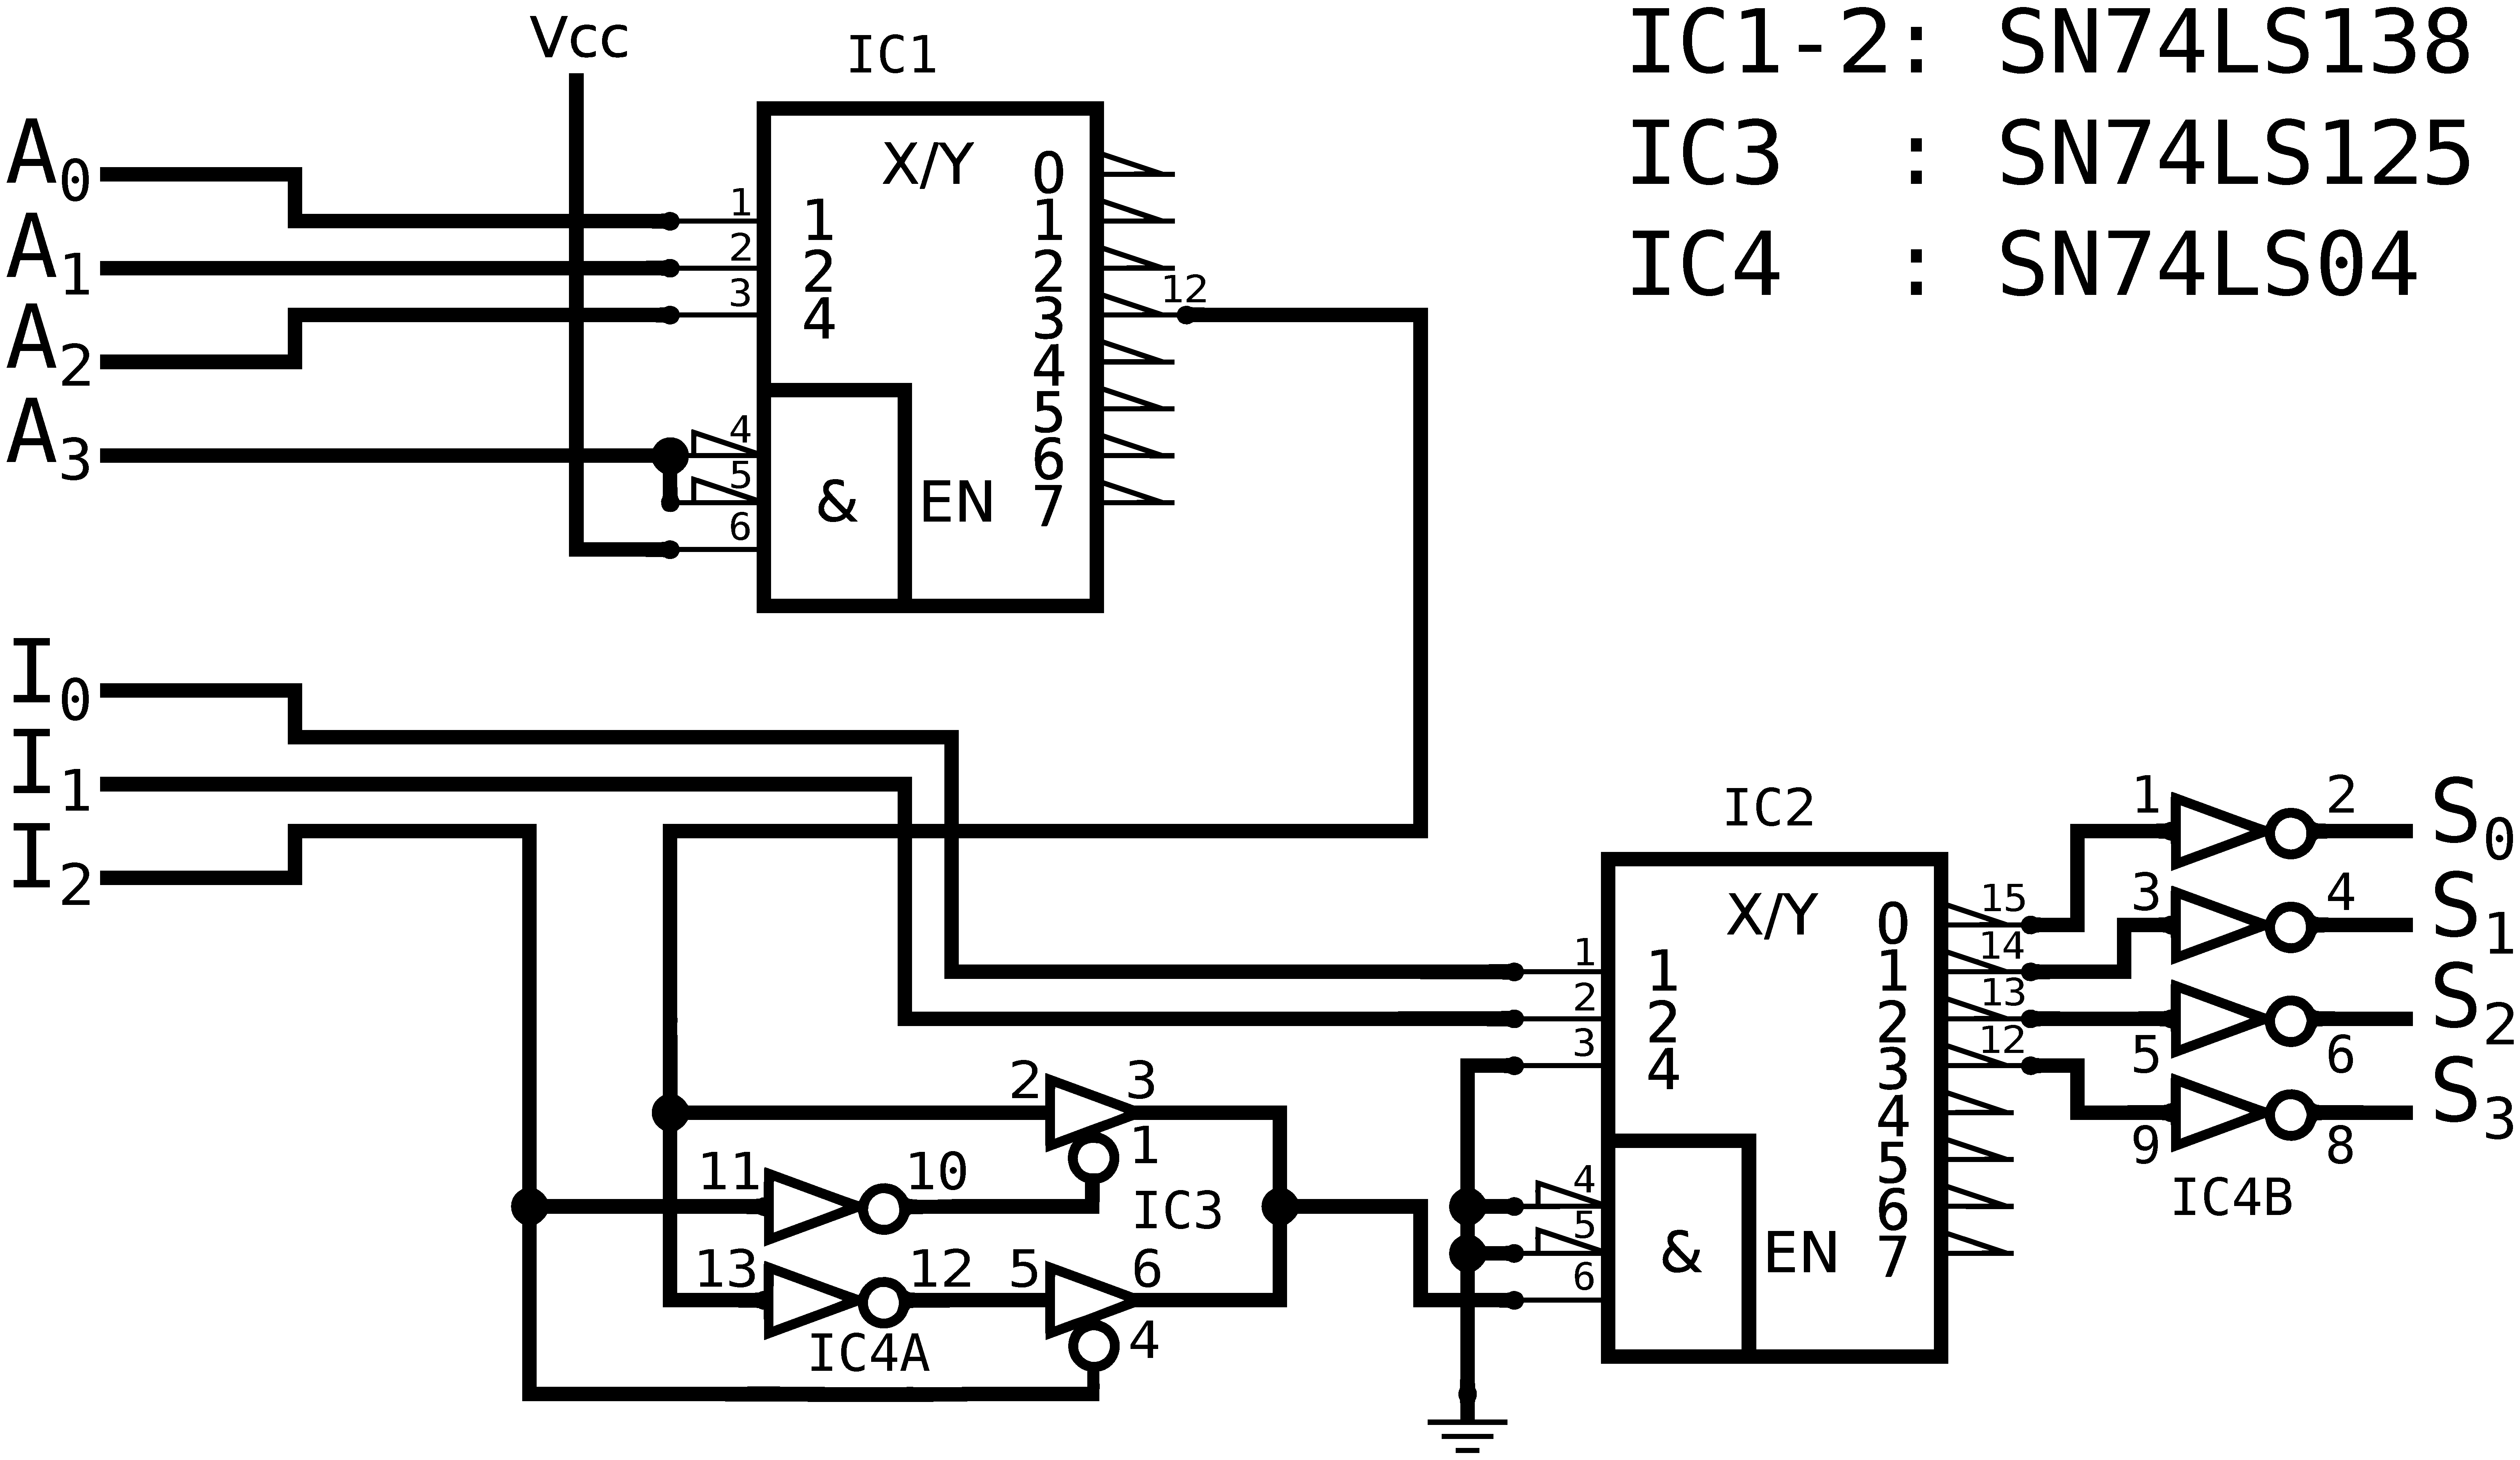
\includegraphics[scale=.1]{esqelect.eps}

\subsection{Transformação das expressões algébricas}

\subsubsection{De forma a serem concretizadas com portas NAND-2, NAND-3 e NOT}


\section{Montagem e Teste}
\subsection{Montagem}
Montou-se o circuito na {\it breadboard} utilizando os circuitos requisitados.
\subsection{Utilização da Ponta de Prova}
%\vspace*{10\baselineskip}
\pagebreak
\subsection{Teste do circuito}

\begin{table}
\centering
\begin{tabularx}{1.0\textwidth}{|| >{\setlength\hsize{1\hsize}\centering}X  >{\setlength\hsize{1\hsize}\centering}X >{\setlength\hsize{1\hsize}\centering}X >{\setlength\hsize{1\hsize}\centering}X || >{\setlength\hsize{1\hsize}\centering}X >{\setlength\hsize{1\hsize}\centering}X || >{\setlength\hsize{1\hsize}\centering}X  | >{\centering\arraybackslash}X ||}
\hline 
\multicolumn{4}{||c||}{Valores de entrada} & \multicolumn{2}{c||}{Valores Esperados} & \multicolumn{2}{c||}{Valores Obtidos} \\
  \hline
a\textsubscript{3} & a\textsubscript{2} & a\textsubscript{1} & a\textsubscript{0} & f\textsubscript{1} & f\textsubscript{0} & f\textsubscript{1} & f\textsubscript{0} \\ \hline
0   &  0  &  0  & 0   & L  & H  && \\ \hline
0   &  0  &  0  & 1   & L  & H  &&\\ \hline
0   &  0  &  1  & 0   & L  & H  &&\\ \hline
0   &  0  &  1  & 1   & H  & L  &&\\ \hline
0   &  1  &  0  & 0   & L  & H  &&\\ \hline
0   &  1  &  0  & 1   & L  & H  &&\\ \hline
0   &  1  &  1  & 0   & L  & H  &&\\ \hline
0   &  1  &  1  & 1   & L  & H  &&\\ \hline
1   &  0  &  0  & 0   & L  & H  &&\\ \hline
1   &  0  &  0  & 1   & L  & H  &&\\ \hline
1   &  0  &  1  & 0   & L  & H  &&\\ \hline
1   &  0  &  1  & 1   & L  & H  &&\\ \hline
1   &  1  &  0  & 0   & L  & H  &&\\ \hline
1   &  1  &  0  & 1   & L  & H  &&\\ \hline
1   &  1  &  1  & 0   & L  & H  &&\\ \hline
1   &  1  &  1  & 1   & L  & H  &&\\ \hline
\end{tabularx}
\caption{Tabela de Testes das Funções}
\end{table}



\begin{table}
\centering
\begin{tabularx}{1.0
\textwidth}{|| >{\setlength\hsize{1\hsize}\centering}X >{\setlength\hsize{1\hsize}\centering}X >{\setlength\hsize{1\hsize}\centering}X >{\setlength\hsize{1\hsize}\centering}X >{\setlength\hsize{1\hsize}\centering}X || >{\setlength\hsize{1\hsize}\centering}X >{\setlength\hsize{1\hsize}\centering}X >{\setlength\hsize{1\hsize}\centering}X >{\setlength\hsize{1\hsize}\centering}X || >{\centering\arraybackslash}X  | >{\centering\arraybackslash} X | >{\setlength\hsize{1\hsize}\centering}X | >{\centering\arraybackslash}X ||}
\hline 
\multicolumn{5}{||c||}{Valores de entrada} & \multicolumn{4}{c||}{Valores Esperados} & \multicolumn{4}{c||}{Valores Obtidos} \\
  \hline

I\textsubscript{2} & I\textsubscript{1} & 
I\textsubscript{0} & 

f\textsubscript{1} & f\textsubscript{0} & 

S\textsubscript{3} & S\textsubscript{2} & 
S\textsubscript{1} & S\textsubscript{0} &
 
S\textsubscript{3} & S\textsubscript{2} & 
S\textsubscript{1} & S\textsubscript{0} 
\\ \hline
0  & 0  & 0  & X  & 0  & L  & L & L & L &&&& \\ \hline
0  & 0  & 0  & X  & 1  & L  & L & L & H &&&&\\ \hline
0  & 0  & 1  & X  & 0  & L  & L & L & L &&&&\\ \hline
0  & 0  & 1  & X  & 1  & L  & L & H & L &&&&\\ \hline
0  & 1  & 0  & X  & 0  & L  & L & L & L &&&&\\ \hline
0  & 1  & 0  & X  & 1  & L  & H & L & L &&&&\\ \hline
0  & 1  & 1  & X  & 0  & L  & L & L & L &&&&\\ \hline
0  & 1  & 1  & X  & 1  & H  & L & L & L &&&&\\ \hline
1  & 0  & 0  & 0  & X  & L  & L & L & L &&&&\\ \hline
1  & 0  & 0  & 1  & X  & L  & L & L & H &&&&\\ \hline
1  & 0  & 1  & 0  & X  & L  & L & L & L &&&&\\ \hline
1  & 0  & 1  & 1  & X  & L  & L & H & L &&&&\\ \hline
1  & 1  & 0  & 0  & X  & L  & L & L & L &&&&\\ \hline
1  & 1  & 0  & 1  & X  & L  & H & L & L &&&&\\ \hline
1  & 1  & 1  & 0  & X  & L  & L & L & L &&&&\\ \hline
1  & 1  & 1  & 1  & X  & H  & L & L & L &&&&\\ \hline
\end{tabularx}
\caption{Tabela de Teste das Saídas}
\end{table}

\section{Conclusão}
Com este trabalho teve-se como objectivo a concepção e concretização de um
circuito que executa duas funções combinatórias. Para tal utilizou-se os Mapas
de Karnaugh para obter as funções como soma de produtos e também como produto de
somas para que depois fossem facilmente convertidas para expressões com, 
exclusivamente portas NAND e NOT ou NOR e NOT. A partir destas expressões 
escolhemos a mais económica e eficiente de implementar, tendo elaborado o 
respectivo diagrama lógico e esquema eléctrico após selecção dos circuitos 
integrados a usar.

\end{document}

-----------> footnotes
